\chapter{Intensity modulated particle therapy for multiple targets}
\label{chapter:complex}
\minitoc

\section{Introduction}

Lung cancer is the leading cause of cancer-related death, with approximately 160 000 deaths in the U.S. in 2014 \cite{Siegel2014}.
More than half of all patients with lung cancer are diagnosed with stage IV non-small cell lung cancer (NSCLC) \cite{Ramalingam2008, Iyengar2014}.
The prognosis for stage IV NSCLC is poor, with only 12 months median survival after first line chemotherapy \cite{Socinski2013}. 

A stereotactic body radiation treatment (SBRT) shows good results for treating NSCLC \cite{Baumann2009, Fakiris2009, Grutters2010, Greco2011}. 
Furthermore, several studies have shown that SBRT can be used in the setting of limited metastatic 
disease \cite{Rusthoven2009, Villaruz2012, Salama2012, Iyengar2014}. 
Passive scattering particle therapy has also proved as an effective treatment for NSCLC \cite{Grutters2010, Tsujii2012} and it could be considered an alternative
to the standard photon treatment.

It was shown in Chapter~\ref{PatStudy} that scanned carbon ions (PT) could also be used as a treatment modality for NSCLC. One of the conclusions of the study shown in Chapter~\ref{PatStudy} 
was that patients with multiple disease sites would especially benefit from PT compared to SBRT. However, limitations of this study were the small number of patients (4) and
a single-field uniform optimization (SFUD) used for treatment planning. Several vital organs, beside the lungs, need to be considered in the treatment planning for NSCLC patients, such as heart, spinal cord, esophagus and large vessels.
Due to overlapping entry channels SFUD is limited in treating NSCLC, especially in patients with a tumor in close vicinity to an vital organ.
It is not possible to create clinically acceptable treatment plans with SFUD for such complex geometry.

We hypothesize that intensity modulated particle therapy (IMPT), permits to calculate adequate treatment plans. Furthermore, IMPT 
should be able to provide a single fraction scheme in patients, where SBRT is limited by OAR constraints. 

The treatment of lung cancer patients  with multiple disease sites was investigated using a state of the art 4D IMPT optimization. 
Treatment plans were generated with two different 4D optimization techniques and compared with SBRT plans, which were actually used for the treating patients.


%A simple geometrical union of target contour in different CT states, geo-ITV, leads to poor 4D dose distribution, when treating moving tumors with particle therapy \cite{Rietzel2010}.
\newpage
\section{Materials and Methods}

The 4D extension of GSI's treatment planning system TRiP98 \cite{Kraemer2000a, Richter2013} was used and modified to create the needed treatment plans. A description of the modifications and tools used will be given here, 
alongside with the patient data.

\subsection{Patient data}


In this study, 8 patients with 2 - 5 lung metastases, summing up to 24 metastases in total, were included. The median lesion size was 4.2 cm$^3$ (25-75\% 2.4 - 22.2) and the median peak-to-peak motion was 5.9 mm (2.7 - 8.1). 
Further details are given in Table~\ref{tab:patdata2}.
The target motion and PT treatment planning were based on a 4D-CT, consisting of 10 phases (0 - 9), with phase 0 (end-inhale) chosen as a reference phase.
A registered positron emission tomography (PET) scan was used to delineate the clinical target volumes (CTV). 

Patients 1 - 3 had no OAR in CTV vicinity (closer than 10 mm), while patients 4 - 8 had at least one.

All patients were treated with SBRT at the Chamaplimaud Center for the Unknown, Lisbon (Portugal), with different fraction schemes. 
The number of fractions and doses delivered are given in Table~\ref{tab:patdata2}.

\newpage


\begin{table}[H]
	\centering
	%   \footnotesize
	\caption{Target characteristics, with CTV volumes, peak-to-peak motions, fractionation schemes and number of fields used for PT treatment planning. Last column 
	shows which OARs were present in the target vicinity (closer than 10 mm). SA stands for smaller airways and esoph. for esophagus.}
	\begin{tabular}{c|c|c|c|c|c|c}
		\hline\hline
		\multirow{2}{*}{Patient} & \multirow{2}{*}{Target} & \multirow{2}{*}{Volume (cm$^3$)} & Peak-to-peak & Fractionation & Number & OAR in \\
		 & & & motion [mm] & scheme & of fields & proximity \\
		\hline
		\multirow{2}{*}{1} & a & 10.2 & 3.4  & 1 x 24 Gy & 2 & \\
		 & b & 14.4 & 2.8 & 1 x 24 Gy  & 2 &  \\

		 
		 \hline
		 \multirow{5}{*}{2} & a & 3.8 & 5.8  & 1 x 24 Gy & 2 &\\
		  & b & 4.3 & 0.8  & 1 x 24 Gy& 2 &\\
		  & c & 2.7 & 3.4  & 1 x 24 Gy & 2&\\
		  & d & 3.1 & 2.1  & 1 x 24 Gy & 2&\\
		  & e & 0.5 & 0.5  & 1 x 24 Gy & 2&\\
		  \hline
		  \multirow{2}{*}{3} & a & 139 & 0.6 & 1 x 24 Gy & 3 \\
		 & b & 9.2 & 2.0  & 1 x 24 Gy & 2 \\
		 \hline
		 \multirow{2}{*}{4} & a & 4 & 9  & 3 x 9 Gy  & 5 & SA, esoph., heart \\
		 & b & 0.8 & 7.8  & 1 x 24 Gy & 2 \\
		 \hline
		 \multirow{4}{*}{5} & a & 3.4   & 5  & 1 x 24 Gy & 3 &  \\
				    & b & 2.4 & 4.4  & 1 x 24 Gy & 2 &\\
				    & c & 2.0 & 6.3  & 1 x 24 Gy& 2& Heart\\
				    & d & 2.4 & 6.4  & 1 x 24 Gy & 2 & Heart\\
		\hline	    
		\multirow{2}{*}{6} & a & 20.6 & 7.4 & 1 x 24 Gy & 4 & SA  \\
		 & b & 27.1 & 6.0  & 1 x 24 Gy &5 & SA  \\
		 
		 \hline
		 \multirow{2}{*}{7} & a & 2.3 & 12  & 1 x 24 Gy & 2 &\\
		 & \multirow{2}{*}{b} & \multirow{2}{*}{0.4} & \multirow{2}{*}{11.8}  & \multirow{2}{*}{5 x 7 Gy} & \multirow{2}{*}{5} & Heart, esoph., \\
		 & & & & & & stomach \\
		 \hline
		 \multirow{5}{*}{8} & a & 136 & 12  & 3 x 9 Gy & 2 & Heart\\
		  & b & 12.4 & 2.5  & 1 x 20 Gy & 2 &\\
		  & c & 123 & 14  & 3 x 9 Gy & 2  &Heart \\
		 & d & 80.7 & 17  & 1 x 22 Gy & 3  &\\
		 & e & 86.7 & 6.6  & 1 x 20 Gy & 3 & SA \\
		\hline\hline
	\end{tabular}
	\label{tab:patdata2}
\end{table}


\newpage

\subsection{Multiple targets}

The TRiP98 optimization works on minimizing the residual of a nonlinear equation system \cite{Kraemer2000a}. The cost function $E(N)$ for the particle number $\vec{N}$ is given by  :
\begin{equation}
\label{eq-costFunc}
 E(\vec{N}) = \sum_{i\in T} \left( D_{plan}^{i} - D_{act}^{i}(\vec{N})\right) +  \theta(D_{act}-D_{max})w_{OAR}\sum_{j\in OAR} \left( D_{act}^{i}(\vec{N}) - D_{Max} \right)
\end{equation}

For a CT voxel $i$ and $j$ in the target $T$ and the OAR, respectively; $ D_{plan}$, $D_{act}$ and $D_{max}$ are the planned, actual and maximum allowed dose, respectively; $\theta$ is the 
Heaviside step function and $w_{OAR}$ is an OAR specific weight.

The $D_{act}(\vec{N})$ is calculated as
\begin{equation}
 D_{act}(\vec{N}) = \sum_{k=1}^n RBE(N) c_{ik}N 
\end{equation}

The coefficient $c_{ik}$ gives the dose deposition at a voxel $i$ of a pencil beam $k$, 
with $n$ being the number of pencil beams and RBE is the relative biological effectiveness, calculated with the local effect model or LEM \cite{Elsaesser2010} . 

There is no restriction for the number of targets or fields in the minimizing function, so the first part of Eq.~\ref{eq-costFunc} can be expanded to:

\begin{equation}
\label{eq-multiCost}
 E(\vec{N}) = \sum_{T} \sum_{i\in T} \left( D_{plan}^{i,T} -\sum_{k=1}^n c_{ik}N\right)
\end{equation}

However, the setup of raster points in TRiP98 allowed only one target. It was therefore expanded in a way that a field was designated to a specific target, as displayed in Fig~\ref{Fig:multiTargets}. 
Raster points for each field are created only around the designated target. All fields contribute dose to all voxels in the optimization. Specifically, $k$ in Eq.~\ref{eq-multiCost} runs over all pencil beams. 
Because the optimization function was not changed, 
all TRiP98 4D functionalities could be used, as explained in the next sections.




\newpage


\begin{figure}[H]
	\begin{center}
		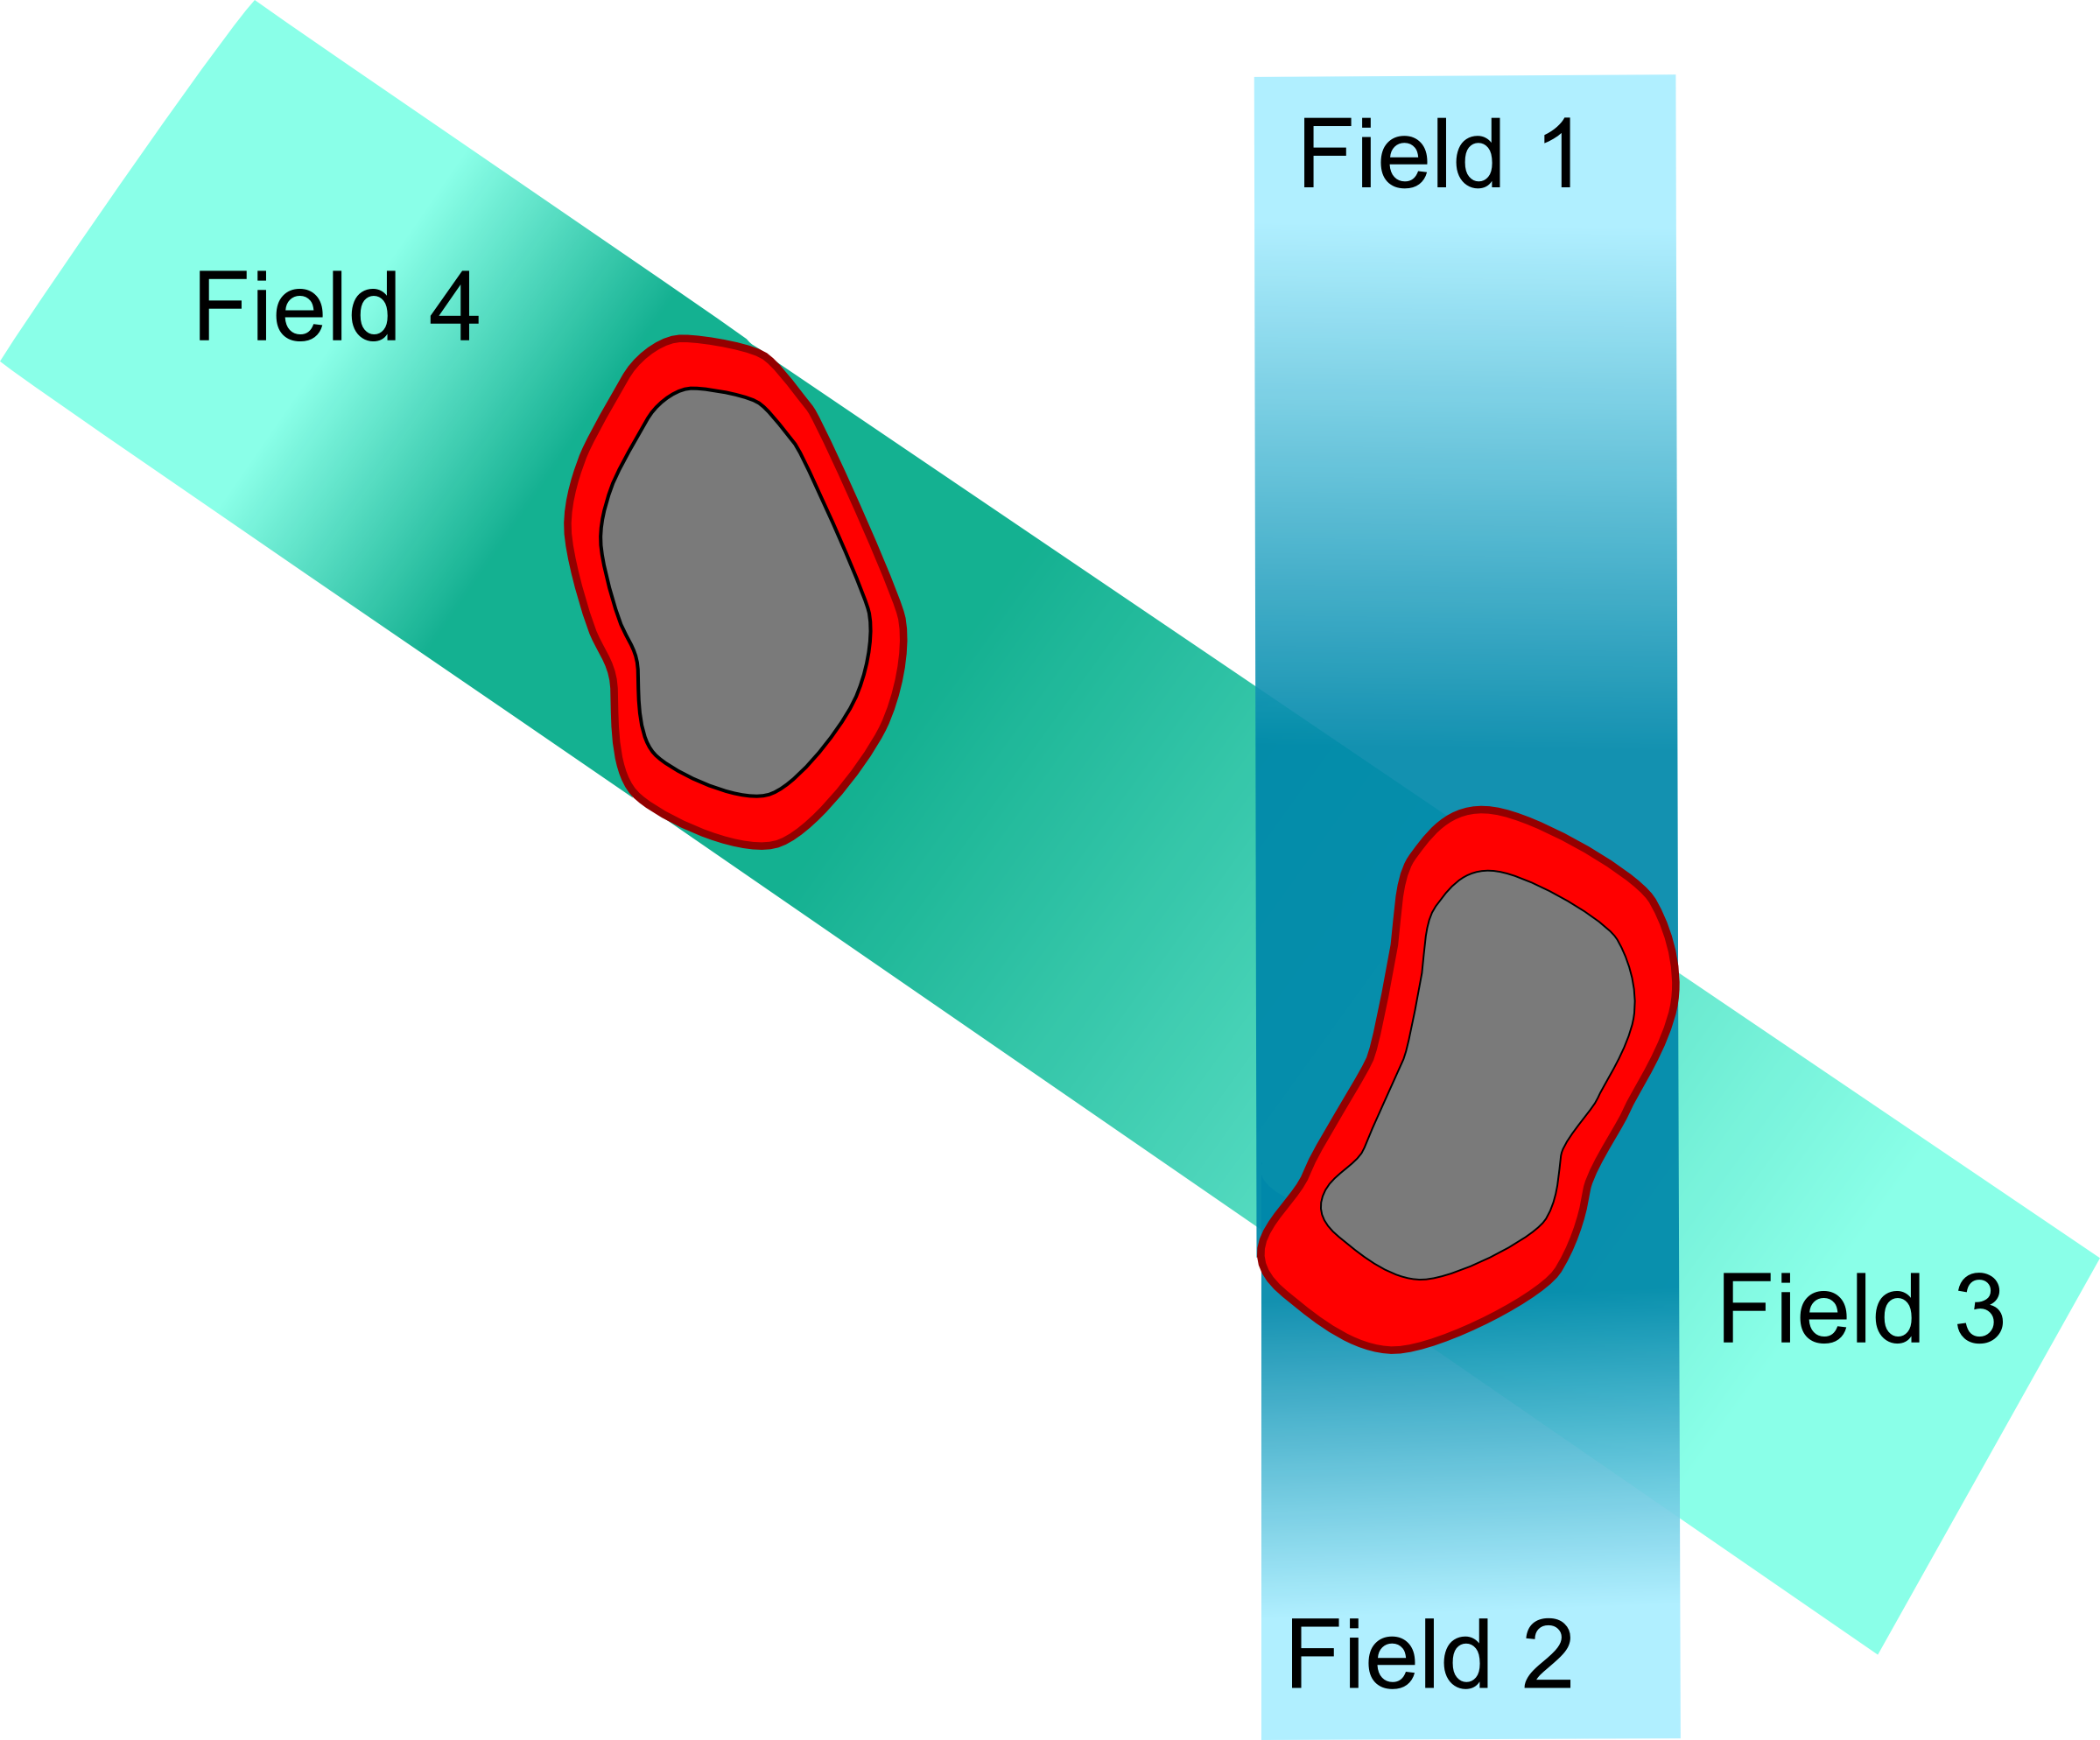
\includegraphics[width=1\textwidth]{./ComplexPatients/Images/multiTarget.png}
		\caption{Optimization of multiple targets. (a) Fields 1 and 2 are designated to target T1 and fields 3 and 4 to target T2. 
		Optimization takes into account all target voxels and contributions from all fields. An example is shown in (b) and (c), where targets
		were optimized individually (b) and together (c). The dose in (b) reaches almost 200\% in the healthy tissue.}
		\label{Fig:multiTargets}
	\end{center}
\end{figure}



\subsection{Optimization techniques}

Investigation of two different optimization techniques to handle range changes in moving tumors was made. For each patient, two sets of plans were created: a field-independent ITV (ITV) and a 4D optimization (4Dopt). 

\begin{itemize}
\item \textbf{Field-independent ITV:} The water-equivalent path length ITV (WEPL-ITV) is different for each field, creating unnecessary margins when combining 
WEPL-ITV from different fields (see Fig.~\ref{Fig:weplITV}a). 
Graeff et. al \cite{Graeff2012} proposed a solution to include range margins into the field description itself, instead of creating a bigger PTV. 

Thus, all fields have the same target in the optimization, permitting simultaneous optimization. 
Treatment plans were made for all targets with IMPT on a ITV in the reference phase. Additionally the target in motion state 5 (end-exhale) was included in the optimization
to make the plan more robust against range changes in different motion states.

\item \textbf{4D Optimization:} To include WEPL change specific to each motion state, a 4D optimization was used. 4Dopt uses a WEPL-ITV for raster setup, 
however the actual optimization is performed on each target voxel in each motion state $m$. The optimization function thus changes to \cite{Graeff2012}:

\begin{equation}
E(\vec{N}) = \sum_{m=1}^{M}\sum_{T_m} \sum_{i\in T_m} \left( D_{plan}^{i} -\sum_{k=1}^n c_{ikm}N\right)
\end{equation}

All targets were treated with IMPT and 4D optimization. Due to the large optimization problem for targets 3a - b, 5a - d, 6b, 8a and 8c (targets had a big volume or 
OARs were included besides targets in the optimization), a subset of motion states was used in optimization \cite{Graeff2012}. 
To cover most of the different tumor positions, two extreme motion states (0 and 5) and an intermediate position (7) were chosen.

\end{itemize}

The same number of fields and the same field angles were used in both techniques.

To reduce the optimization problem, only selected large OARs, such as the heart or the esophagus, were used. Large OARs were manually cropped to the region close to the 
target. The dose, however, was calculated on the whole OAR to ensure the validity of results.

For targets with different fractionation scheme (targets 8a-e), TRiP98 was modified to include an option, allowing specific dose fractions for specific targets.


\begin{figure}[H]
	\begin{center}
		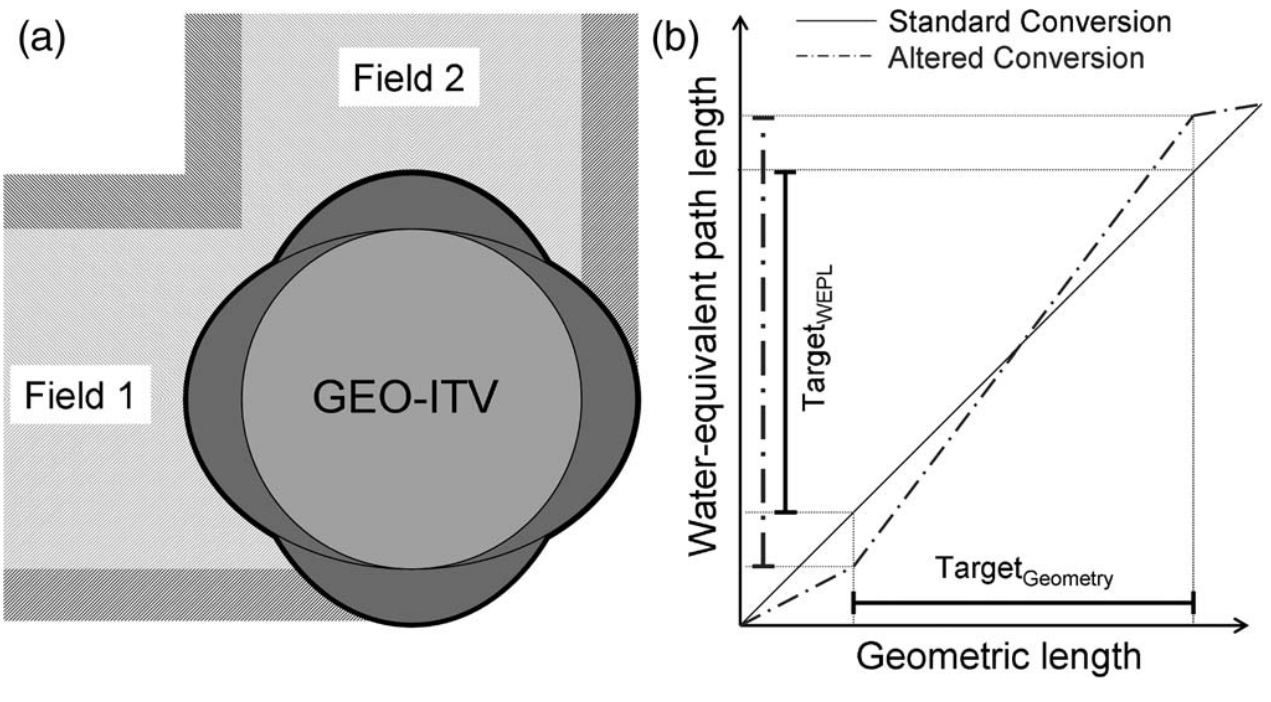
\includegraphics[width=0.7\textwidth]{./ComplexPatients/Images/weplITV.png}
		\caption{A schematic presentation of the ITV. (a) The dark gray ellipses show the margins needed for specific fields to account for range changes in different motion states.
		When a common target volume for two perpendicular fields is generated (v black contour) it creates unnecessary lateral extension of both fields, as shown by the dark gray
		entry channels. A solution is shown in (b). Rather than using standard, geometric margins, both fields use the same geometry, however the conversion of geometry to WEPL
		is altered for each field. The plot in (b) shows the standard (solid line) and an altered conversion (dashed-doted line) for a beam passing a homogeneous CTV. The altered conversion
		increases the WEPL extent and thus implicitly increasing margins for a single field only. Figure taken from \cite{Graeff2012}}
		\label{Fig:weplITV}
	\end{center}
\end{figure}

\subsection{Treatment planning}

An isotropic margin of 3 mm was added to each CTV to account for uncertainties in treatment delivery. 
A WEPL-ITV was constructed on the CTV with margins for each individual field, which was than used either in the optimization (ITV)
or for the raster setup (4Dopt). Due to large memory demands, the targets in each lung were optimized separately. 
  
The planning objective was 99\% of each target volume should receive at least 100\% of the planned dose (D$_{99}$\% $\geq$ 100\%). Two dose limitation were used for OARs, as defined in 
the AAPM task group \cite{Benedict2010}. The first limitation was the maximum dose to a single voxel $D_{Max}$ and the second the maximum dose deposited to a 
specific OAR volume $D_{Threshold}$. All limits are summarized in Table~\ref{tab:oarlimits}.
 
After the optimization the 4D-dose was calculated for two motion periods (3.6 sec and 5.0 sec) and two starting phases (0$^\circ$ and 90$^\circ$) as explained in Section~\ref{PTTP}. 
The relative biological effectiveness (RBE) was calculated with LEM IV \cite{Elsaesser2010}. 
Alpha beta ratio of 6 and 2 was used for the target and normal tissue, respectively.

The motion was mitigated by applying slice-by-slice rescanning to each plan. 
The number of rescans was limited by the number of particles in a single raster point, which should not be lower than 8000 due to the
monitoring precision. The maximum number of rescans was limited to 20.

A detailed explanation of the SBRT treatment planning is given in Section~\ref{SBRTTP}.

For patients 4 - 7 OAR doses could not be sufficiently reduced in optimization. It was necessary to add margins to the OAR and then 
subtract the OAR plus margins from the target. For SBRT the OAR plus margins was subtracted from PTV, which included 3 mm isotropic margins on a geometrical ITV. 
In PT geometrical ITV was not used, so in each of the 10 motion states, OAR plus margins was subtracted from CTV plus 3 mm. 

In the first try the OAR was included in the optimization with different weights ($w_{OAR}$ in Eq~\ref{eq-costFunc}) and without any subtraction from the target. 
For any 3D treatment plan with an acceptable dose distribution after the optimization, a 4D dose was calculated and OAR and target dose were inspected. If the plan was rejected, the optimization was repeated, adding the OAR subtraction from the target volume. 



\subsection{Dose escalation}

A single fraction of 24 Gy could not be used in SBRT treatment for targets 4a, 7b and 8a-e due to OAR dose constraints. For these targets additional 
PT plans were generated with 1 x 24 Gy fractionation scheme, in order
to estimate if PT could respect OAR constraints for these targets, while delivering 1 x 24 Gy. 

\subsection{Data evaluation}

For a comparison of the target coverage, the minimum dose in 99\% of the target volume ($D_{99\%}$) was evaluated. $D_{Max}$ and $D_{Threshold}$ were used in the OAR dose comparison. $D_{Max}$ and $D_{Threshold}$ were normalized to the respective limits
in the fractionation scheme used, see Table~\ref{tab:oarlimits}. Additionally, the volume receiving 20\% of the planned dose ($V_{20\%}$) was used to assess the ipsilateral lung dose.

Paired t-tests were performed to compare the dose metrics mentioned between SBRT, ITV and 4Dopt. A p-value < 0.05 was considered as significant. 

\section{Results}

An example of different treatment plans for three patients are shown in Fig.~\ref{Fig:multiExample}. 

\newpage
\begin{figure}[H]
	\begin{center}
		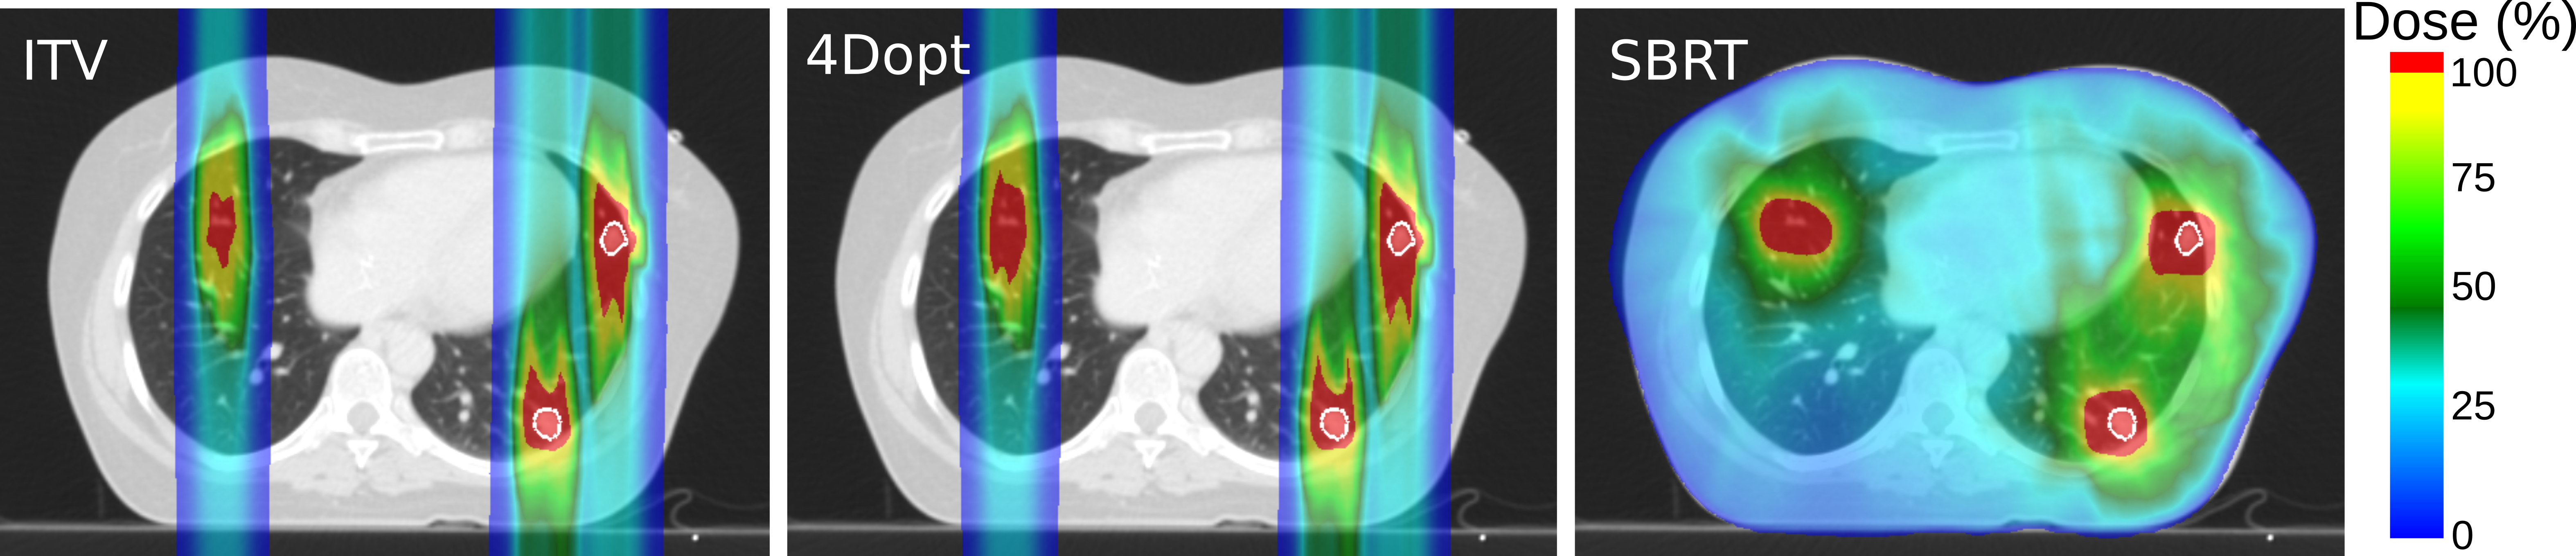
\includegraphics[width=0.9\textwidth]{./ComplexPatients/Images/multiExample.png}
		\caption{Treatment plans for ITV (left), 4Dopt (middle) and SBRT (right) for patients 2 (top), 7 (middle) and 8 (bottom). 
		CTV, heart, esophagus and stomach contours are outlined in white, red, blue and orange,
		respectively. The patient 7 image is magnified to the target 7b location. Patient 2 has 5 disease sites with no OARs in target vicinity. Patient 7 had poor target coverage
		with PT due to a large target motion and OAR proximity. A 1 x 24 Gy plan could be generated for patient 8 with PT, 
		while SBRT was limited by the dose deposited in the heart. Therefore the fractionation scheme was adapted and 2 targets were treated with 3 x 9 Gy, 2 with 1 x 20 Gy and one with 1 x 22 Gy. }
		\label{Fig:multiExample}
	\end{center}
\end{figure}
\newpage
\subsection{Target Coverage}

The results for CTV $D_{99\%}$ for all patients are shown in Table~\ref{tab:resultsComplex}. All SBRT plans were approved by a physician, 
even though the prescribed dose for patients 4 - 6 was not met due to an OAR proximity. Target 7b $D_{99\%}$ for PT was below prescription and SBRT delievered full dose.
Average CTV $D_{99\%}$ was 97, 95 and 98\% for ITV, 4Dopt and SBRT, respectivelly, There was a significant difference between ITV and 4Dopt and SBRT and 4Dopt.
% Excluding patients 4 - 7, there were 1 and 5 cases (out of 128) of too low CTV dose across different
% motion types for ITV and 4Dopt, respectively. For patients 4 - 6 ITV and 4Dopt had higher CTV $D_{99\%}$ than SBRT, except for target 5c and 4a for ITV.
% The lowest CTV $D_{99\%}$ was 75\% for target 7b.

% There was no significant difference in CTV $D_{99\%}$ between SBRT, ITV and 4Dopt.

\begin{table}[H]
	\centering
	%   \footnotesize
	\caption{CTV $D_{99\%}$ for tITV, 4Dopt and SBRT for 8 patients. The results for ITV and 4Dopt are shown as median (range) across the different motion types.}
	\begin{tabular}{c|c|c|c|c}
		\hline\hline
		\multirow{2}{*}{Patient} & \multirow{2}{*}{Target} & \multicolumn{3}{|c}{CTV $D_{99\%}$ (\%)}  \\
		 &  & ITV & 4Dopt & SBRT \\
		 \hline
		 
\multirow{2}{*}{1} & a & 101.0(101.0 - 101.0) & 101.0(101.0 - 101.0) & 100.0\\ 
 & b & 101.0(101.0 - 102.1) & 101.0(101.0 - 101.0) & 100.0\\ 
 \hline
\multirow{5}{*}{2} & a & 101.0(101.0 - 102.1) & 100.0(99.0 - 102.1) & 106.3\\ 
 & b & 102.1(102.1 - 102.1) & 102.1(102.1 - 102.1) & 103.1\\ 
 & c & 101.0(100.0 - 101.0) & 101.6(101.0 - 102.1) & 104.2\\ 
 & d & 102.1(101.0 - 102.1) & 102.1(102.1 - 102.1) & 107.3\\ 
 & e & 101.0(101.0 - 101.0) & 101.0(101.0 - 102.1) & 108.3\\ 
 \hline
\multirow{2}{*}{3} & a & 101.0(101.0 - 101.0) & 101.0(101.0 - 101.0) & 101.0\\ 
 & b & 98.4(97.9 - 99.0) & 97.9(97.9 - 97.9) & 102.1\\ 
 \hline
\multirow{2}{*}{4} & a & 65.3(63.9 - 69.4) & 70.4(68.5 - 72.2) & 66.7\\ 
 & b & 101.0(100.0 - 102.1) & 100.5(100.0 - 102.1) & 103.1\\ 
 \hline
\multirow{4}{*}{5} & a & 100.0(99.0 - 101.0) & 100.0(100.0 - 100.0) & 101.0\\ 
 & b & 101.6(100.0 - 102.1) & 97.9(96.9 - 99.0) & 101.0\\ 
 & c & 95.3(94.8 - 96.9) & 94.3(92.7 - 94.8) & 99.0\\ 
 & d & 99.0(97.9 - 99.0) & 99.5(99.0 - 100.0) & 94.8\\ 
 \hline
\multirow{2}{*}{6} & a & 89.1(88.5 - 90.6) & 85.4(85.4 - 87.5) & 69.8\\ 
 & b & 78.6(77.1 - 79.2) & 72.4(71.9 - 72.9) & 69.8\\ 
 \hline
\multirow{2}{*}{7} & a & 102.1(102.1 - 102.1) & 99.0(99.0 - 99.0) & 101.0\\ 
 & b & 83.9(82.1 - 85.7) & 75.0(75.0 - 75.0) & 100.0\\ 
 \hline
\multirow{5}{*}{8} & a & 100.0(100.0 - 100.9) & 99.5(99.1 - 100.9) & 105.6\\ 
 & b & 101.3(100.0 - 102.5) & 100.0(100.0 - 101.3) & 105.0\\ 
 & c & 100.0(99.1 - 100.0) & 99.5(97.2 - 100.0) & 106.5\\ 
 & d & 102.3(102.3 - 102.3) & 89.8(89.8 - 90.9) & 102.3\\ 
 & e & 102.5(102.5 - 102.5) & 91.9(91.3 - 92.5) & 101.3\\ 
 \hline

\hline\hline
	\end{tabular}
	\label{tab:resultsComplex}
\end{table}
\newpage
\subsection{Dose in OARs}

$D_{Max}$ and $D_{Threshold}$ for 8 OARs are shown in Table~\ref{tab:OARComplex}. Dose volume histograms (DVH) for patients 4, 6 and 7 are shown in Fig.~\ref{Fig:dvh}.
There was a significant difference between PT and SBRT in $D_{Max}$ and $D_{Threshold}$ 
for heart, spinal cord, esophagus and aorta. No significant difference was observed for $D_{Max}$ and $D_{Threshold}$ in the smaller airways.
No significant difference was observed in the dose to any OAR between the different motion types or between ITV and 4Dopt.
The overall OAR difference for patients between SBRT and ITV
was significant, 17 (4 - 52)\% and 27 (8 - 55)\% of OAR limits for $D_{Max}$ $D_{Threshold}$, respectivelly.
The ipsilateral lung $V_{20\%}$ was 14.5(0.0 - 48.7), 14.4(0.0 - 43.7) and 29.8 (5.8 - 89.2)\% for ITV, 4Dopt and SBRT, respectively. Both, ITV and 4DITV ipsilateral lung $V_{20\%}$ was
significantely different from SBRT.

The margins used for the OAR subtraction for PT and SBRT can be found in Table~\ref{tab:oarmargins}.

All treatment plans exceeded the $D_{Max}$ limit for the smaller airways in patients 4, 6 and 8 and for the heart in patient 6. 
Additionally, the SBRT esophagus and heart $D_{Max}$ limits were exceeded in patients 4 and 8, respectively.


\begin{table}[H]
	\centering
	%   \footnotesize
	\caption{OAR $D_{Max}$, $D_{Threshold}$ and ipsilateral lung $V_{20\%}$ of all patients for ITV, 4Dopt and SBRT. There was a significant difference between PT and SBRT for all OARs, except
	smaller airways' $D_{Max}$. $D_{Max}$ and $D_{Threshold}$ doses are normalized to the corresponding OAR limits in the fractionation scheme used (see \cite{Benedict2010}). 
	The data is displayed as median (range).}
	\begin{tabular}{c|c|c|c}
		\hline\hline
		 
		OAR &  ITV & 4Dopt & SBRT \\
		\hline
		& \multicolumn{3}{c}{$D_{Max}$ (\%)}  \\
		\hline
heart        & 62.0(0.0 - 100.0) & 59.5(0.0 - 97.0) & 82.5(20.0 - 103.0)\\ 
spinalcord    & 13.0(0.0 - 48.0) & 12.0(0.0 - 55.0) & 60.0(21.0 - 79.0)\\ 
smaller airways & 72.5(0.0 - 130.0) & 71.0(0.0 - 117.0) & 72.5(0.0 - 171.0)\\ 
esophagus      & 9.0(0.0 - 79.0) & 8.0(0.0 - 99.0) & 70.5(20.0 - 101.0)\\ 
aorta         & 17.5(8.0 - 61.0) & 15.0(7.0 - 61.0) & 45.0(15.0 - 74.0)\\ 
\hline\hline
& \multicolumn{3}{c}{$D_{Threshold}$ (\%)} \\
\hline
heart & 15.5(0.0 - 59.0) & 16.0(0.0 - 53.0) & 62.5(19.0 - 98.0)\\ 
spinalcord & 11.0(0.0 - 45.0) & 10.0(0.0 - 53.0) & 66.5(28.0 - 95.0)\\ 
smaller airways & 28.0(0.0 - 97.0) & 26.5(0.0 - 89.0) & 68.5(0.0 - 99.0)\\ 
esophagus & 1.0(0.0 - 17.0) & 1.0(0.0 - 20.0) & 49.0(17.0 - 99.0)\\ 
aorta & 5.5(0.0 - 30.0) & 5.5(0.0 - 28.0) & 34.5(12.0 - 59.0)\\ 
\hline\hline
& \multicolumn{3}{c}{$V_{20\%}$ (\%)} \\
\hline
ipsilateral lung & 14.5(0.0 - 48.7) & 14.4(0.0 - 43.7) & 29.8(5.3 - 89.2)\\ 
\hline\hline
	\end{tabular}
	\label{tab:OARComplex}
\end{table}

% \begin{table}[H]
% 	\centering
% 	%   \footnotesize
% 	\caption{$D_{Max}$ and $D_{Threshold}$ for OAR in CTV vicinity for ITV, 4Dopt and SBRT. The rightmost column shown allowed doses,
% 	as defined in \cite{Benedict2010}.}
% 	\begin{tabular}{c|c|c|c|c}
% 		\hline\hline
% 
%  \multicolumn{5}{c}{Patient 1} \\ 
% SmallerAirways & 20.6(20.5 - 21.0) & 24.8(24.5 - 25.0) & 17.5& 13.3\\ 
% Esophagus & 23.0(22.3 - 23.5) & 23.3(23.0 - 23.5) & 25.5& 15.4\\ 
% Heart & 28.0(28.0 - 28.3) & 28.1(28.0 - 28.5) & 29.3& 22\\ 
%  \multicolumn{5}{c}{Patient 4} \\ 
% Heart & 22.8(22.3 - 23.3) & 23.1(22.0 - 24.3) & 22.8& 22\\ 
%  \multicolumn{5}{c}{Patient 5} \\ 
% AirwaysSmallR & 18.4(17.5 - 19.0) & 18.8(18.5 - 19.0) & 15.3& 0\\ 
% AirwaysSmallL & 22.5(21.8 - 23.3) & 18.0(17.8 - 18.3) & 25.5& 0\\ 
%  \multicolumn{5}{c}{Patient 7} \\ 
% SmallerAirways & 21.3(21.0 - 21.8) & 20.3(19.8 - 20.3) & 16.0& 13.3\\ 
% Heart & 29.8(29.5 - 30.0) & 29.5(29.3 - 29.5) & 30.5& 22\\ 
% 
% \hline\hline
% 	\end{tabular}
% 	\label{tab:OARComplex}
% \end{table}

\newpage
\begin{figure}[H]
	\begin{center}
		\includegraphics[width=0.9\textwidth]{./ComplexPatients/Images/DVH_legend.png}
		\caption{Dose volume histograms for targets 4b, 6a, 6b and 7b with relevant OARs. SBRT, ITV and 4DITV are represented by solid, dashed and dotted lines, respectively. The targets are displayed
		in grayscale, while the OAR colors are shown in legend. SA stands for smaller airways.}
		\label{Fig:dvh}
	\end{center}
\end{figure}
\newpage


\subsection{Dose escalation}

With in PT the 1 x 24 Gy fractionation scheme could be used for targets 8a-e, violating only $D_{Max}$ for the smaller airways (180\%) and the heart (110\%), to
a similar extent as was found acceptable in SBRT.
The SBRT for patient 8 was limited by the heart $D_{Max}$ and $D_{Threshold}$ which were 102\% and 93\%, respectively. SBRT delivered a mean heart dose of 
3 Gy in a single fraction (out of three), whereas PT's mean heart dose was 0.8 Gy.
The difference in the heart dose can be seen in Fig~\ref{Fig:heartDVH}.

For targets 4a and 7b the 1 x 24 Gy fractionation scheme could not be generated with PT. Either the target coverage was low (CTV $D_{99\%} < 50\%$) or the
esophagus $D_{Max}$ and additionally the stomach $D_{Max}$ for target 7b were exceeded.


\begin{figure}[H]
	\begin{center}
		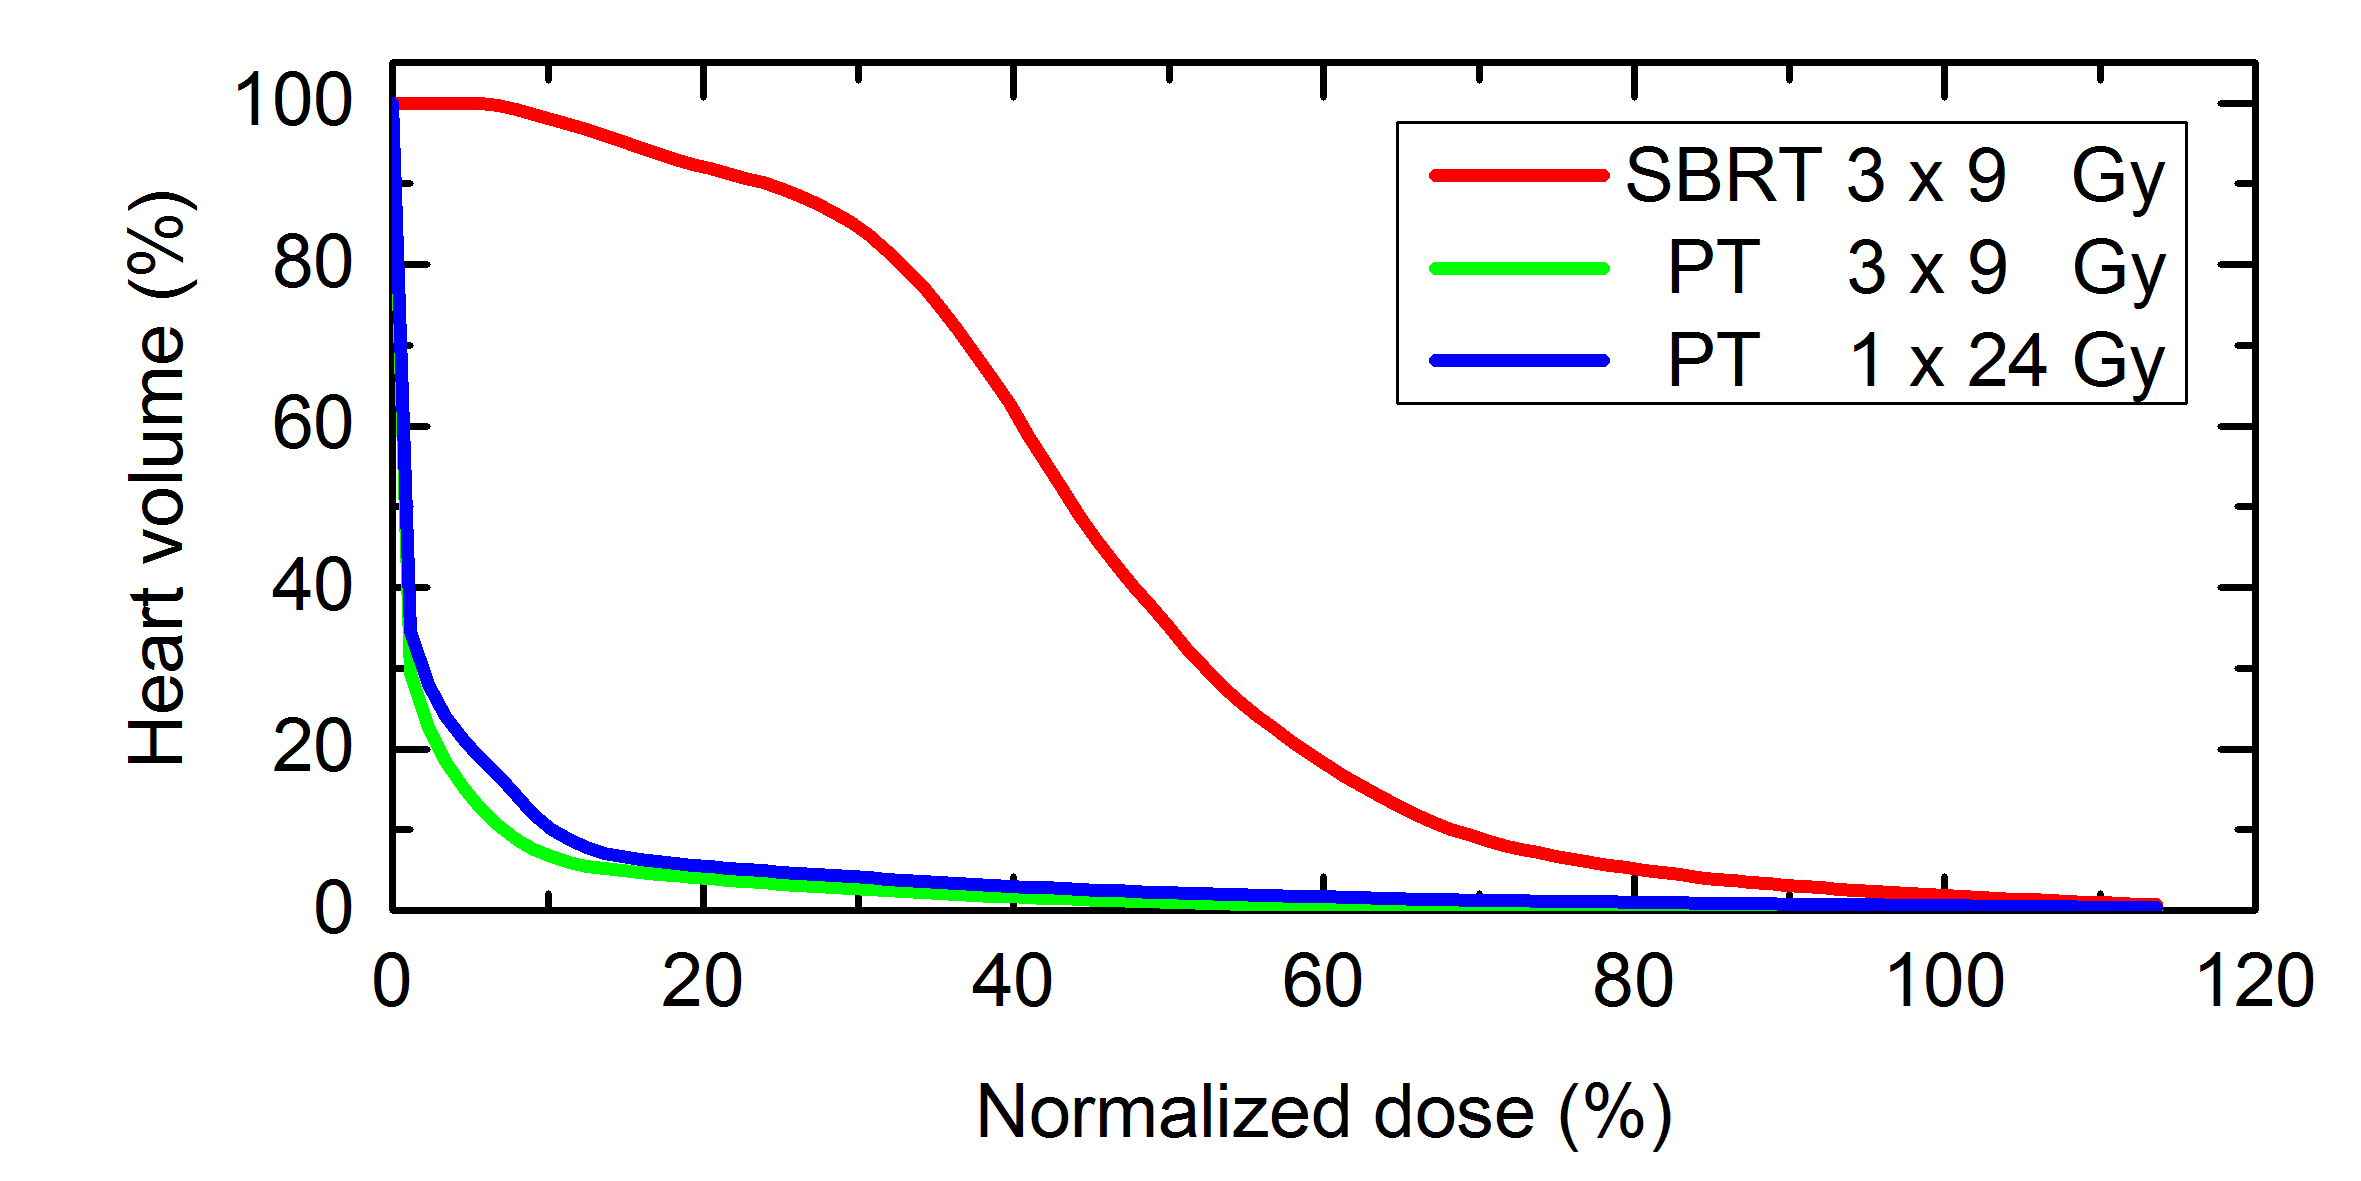
\includegraphics[width=0.9\textwidth]{./ComplexPatients/Images/HeartDVH.png}
		\caption{Dose volume histogram for the heart dose of the Patient 8. SBRT (red) plan was delievered in a 3 x 9 Gy fractionation scheme. The ITV
		 PT plans were generated for the same fractionation scheme (green) and with a dose escalation 1 x 24 scheme (blue). The dose was normalized 
		 to $D_{Max}$ heart limit in respective fractionation scheme - 30 Gy in 3 x 9 Gy and 22 Gy in 1 x 24 Gy.}
		\label{Fig:heartDVH}
	\end{center}
\end{figure}
\newpage

\section{Summary and Discussion}

Clinically valid SBRT plans have been compared to PT treatment plans for NSCLC patients with multiple metastases. 
To the best of our knowledge, this is the first study treating multiple NSCLC metastases with IMPT. A novel approach was used to handle multiple targets, combined
with state of the art 4D IMPT treatment planning. Furthermore, 4D PT doses were calculated for different motion types. 

PT on average delivered less dose to OARs, while still having comparable target coverage to SBRT.
The most important difference was found in the heart dose, with $D_{Threshold}$ being on average 6 times lower in PT compared to SBRT. A recent trial, RTOG 0617, has shown,
that a higher mortality rates could be attributed to higher heart dose for NSCLC patients \cite{Bradley2015}. Furthermore, as seen in Table~\ref{tab:OARComplex}, the median
$D_{Threshold}$ for all OARs is below 30\% and $D_{Threshold}$ exceeds 90\% in only one OAR in one patient. For SBRT $D_{Threshold}$ comes close to the limit in all OARs,
except the aorta. There was no need to include $D_{Threshold}$ in treatment planning, whereas it is imperative in SBRT.

For patients with a complex geometry (4 - 8) PT maintained or even improved target coverage in most cases, while reducing doses to OARs.
The exception was target 7b, where CTV $D_{99\%}$ was low (84\% and 75\% for ITV and 4Dopt, respectively), due to the $D_{Max}$ constraints of the esophagus and the stomach.
The large motion of target 7b (11.8 mm) and the small target volume (0.4 cm$^3$) contributed to a poor PT plan, whereas SBRT was able to deliver the full dose to the target
and adhering to OAR constraints. This supports our claim in Chapter~\ref{PatStudy} that targets with larger volume would benefit most from PT. Furthermore, for small targets
with large motion in OAR vicinity, PT generates worse plans than SBRT. It should be noted, however, that integral doses for all OARs are still lower for PT as seen in Fig~\ref{Fig:dvh}.
The only limitation for PT is usually the OAR's $D_{Max}$.

The biggest advantage of PT could be seen in Patient 8, where the fractionation scheme could be changed to 1 x 24 Gy. 
The large total target volume of Patient 8 could be irradiated with less overall dose and hence significantly reduced the dose to all OARs. Most notably, the heart dose,
which was the limitation factor for SBRT. The difference of 2 Gy mean heart dose in a single fraction is tremendous and could influence the potential outcome for the specific patient.
Again, this confirms our claim of PT benefit for large targets.
Due to the OAR constraints of targets 4a and 7b, located adjacent to important serial organs, no fractionation escalation was possible with PT. 

There was a small difference in the average target coverage between ITV and 4Dopt. The most notable difference was in targets 8d and 8e, where CTV $D_{99\%}$ was 10\% lower
for 4Dopt. For this patient 4Dopt was performed on a subset of the  4D-CT states, which may be inadequate due to the large motion of target 8e (17 mm). In a future study,
the number of voxels included in optimization should be reduced, without reducing the target coverage. A possible solution would be an adaptive dose grid \cite{Prall2016a}.
There was no significant difference between ITV and 4Dopt in the doses to OARs. 
% However, in patients 4 and 6, 4Dopt was able to achieve better target coverage. With ITV, target 4a had worse coverage than 4Dopt and delivered higher dose to 
% smaller airways (see Fig~\ref{Fig:dvh}). For patient 6, 4Dopt deposited less dose to smaller airways in addition to better target coverage.


Even though PT deposits less dose to OARs with the same or even better target coverage, there is still room for improvement in PT 4D treatment planning. 
An implementation of multi-criteria objective planning should bring even better dose distribution and bring possibility to choose between trade-offs \cite{Breedveld2007, Chen2010}. 
Additionally, the multiple target optimization in PT would benefit from a shell around PT where the dose would be minimized. Therefore the excessive dose
in healthy tissue would be further reduced. An introduction of a shell, however, would further enlarge the optimization problem, which is big already for complex geometries 
(patient 4 - 8). An adaptive optimization grid could be a possible solution here as well \cite{Prall2016a}.

In Chapter~\ref{PatStudy} additional range margins to account for range uncertainties could be used in the treatment planning, due to SFUD. 
Because we did not use field specific PTVs, it was not possible to include range uncertainties in this study.
Instead of creating field specific PTVs to include range uncertainties, a solution was proposed to include uncertainties in the optimization process itself \cite{Pflugfelder2008, Unkelbach2009, Fredriksson2011, Chen2012}.
Chen et al. have implemented a robust optimization in a multi-criteria optimization as well \cite{Chen2012}. Furthermore, in a recent treatment planning study by Liu et al. \cite{Liu2016}
a 4D robust optimization was demonstrated, with better results over 3D robust optimization for NSCLC patients. However, only the breathing starting phase was used as an uncertainty,
whereas different motion types should be considered. The disadvantage of 3D and 4D robust optimization is the enlargement of the optimization problem.

Patient 4 $D_{Max}$ esophagus dose ranged over 1.3 Gy across different motion types in 4Dopt, showing the necessity of making treatment plans robust against motion uncertainties, 
especially in the hypo-fractionated regiment. Furthermore, OAR doses that are under the limits after optimization, may exceed them after calculating the 4D dose. 
The ITV and 4Dopt approaches take into account range changes in different motion states, however they do not address interplay. 
This could be solved with a complete 4D optimization \cite{Graeff2013}, where a 4D raster treatment plan is 
generated and each motion state has a designated treatment plan. 

% Clinical application of beam tracking is not yet feasible due to several reasons, such as the 
% inverse interplay, the ion-beam tracking system complexity, precision and speed of the motion monitoring.
% Another solution would be jet-ventilation \cite{Santiago2013}, however, it brings additional complications to treatment.

Apart from 4D robust optimization, the effect of the motion could be minimized by using other motion mitigation techniques, such as gating. Furthermore, gating could improve the target coverage, where the planned dose was
not met. Gating, together with rescanning, has already been successfully implemented clinically for active beam scanning \cite{Rossi2016, Mori2016} and it might be essential to use it in hypo-fractionated 
treatment of moving tumors \cite{Richter2014}.

A recent review showed good local control rates between 66 - 92\% for patients treated with SBRT for in-field recurrent tumors \cite{Amini2014}. 
However, there were grade 4 and 5 complications present. A study by Trovo et al.showed grade 5 pneumonia in
6\% of patients treated \cite{Trovo2014}. As shown in our study, PT delivers less dose to the OARs, ipsilateral lung in particular, and could hence reduce the number of treatment-related
complications.

\section{Conclusions}

PT delivers less dose to OARs compared to SBRT in NSCLC patients with multiple disease sites, while maintaining target coverage. One patient with a large total target volume 
could be irradiated with 1 x 24 Gy, whereas it could not with SBRT. 
There was a small difference between the two 4D treatment planning techniques.

Patients with multiple NSCLC disease site have a poor prognosis, with a median survival shorter than a year. 
A treatment with SBRT can prolong the patient's life, however there is a 10\% chance of death due to the severity of the treatment. PT could
maintain the SBRT survival rate, while tremendously reducing treatment related side effects.